\documentclass[12pt]{article}

\usepackage{url}
\usepackage{fullpage}
\usepackage{amssymb,amsfonts}
\usepackage{amsmath}
\newcommand{\eps}{\varepsilon}
\newcommand{\R}{\mathbb{R}}

\usepackage{listings}
\usepackage{color}
\usepackage{graphicx}

\usepackage{varwidth}

\usepackage{longtable}

\usepackage{hyperref}
\hypersetup{
    linktoc=all,     %set to all if you want both sections and subsections linked
    colorlinks=true,
    linkcolor=blue,
    filecolor=magenta,      
    urlcolor=cyan,
}

\definecolor{dkgreen}{rgb}{0,0.6,0}
\definecolor{gray}{rgb}{0.5,0.5,0.5}
\definecolor{mauve}{rgb}{0.58,0,0.82}

\lstset{frame=tb,
  language=Python,
  aboveskip=3mm,
  belowskip=3mm,
  showstringspaces=false,
  columns=flexible,
  basicstyle={\small\ttfamily},
  numbers=none,
  numberstyle=\tiny\color{gray},
  keywordstyle=\color{blue},
  commentstyle=\color{dkgreen},
  stringstyle=\color{mauve},
  breaklines=true,
  breakatwhitespace=true,
  tabsize=3
}

\usepackage[toc,page]{appendix}

\DeclareMathOperator*{\E}{\mathbb{E}}
\let\Pr\relax
\DeclareMathOperator*{\Pr}{\mathbb{P}}

\DeclareMathOperator*{\Lap}{\text{Lap}}

\DeclareMathOperator*{\Geo}{\text{Geo}}

\def\cl{\lstinline}

\title{CS 208 Homework 4b}
\author{Andrew Shackelford}
\date{April 30, 2019}
\setcounter{tocdepth}{3}

\begin{document}

\maketitle

\textbf{All code and figures are available \href{https://github.com/andrew-shackelford/cs208/tree/master/4b}{here}}.

{
  \hypersetup{linkcolor=black, hidelinks}
  \tableofcontents
}

\newpage

\section{Problem 1}

\subsection{Part A}

\subsubsection{i}

\noindent

For this case, the global sensitivity is $\frac{\infty}{n} = \infty$, since each of the $x_i \in \mathbb{R}$ entries can have values ranging from $-\infty$ to $\infty$ and we are calculating the mean of all the entries.

\subsubsection{ii}

\noindent

For this case, the minimum local sensitivity is $\frac{\infty}{n} = \infty$. Regardless of the ``best case'' dataset, any neighboring dataset can add a value ranging from $-\infty$ to $\infty$, since our universe is the real numbers. This can affect the mean by $\frac{\infty}{n} = \infty$, thus making our minimum local sensitivity $\infty$.

\subsubsection{iii}

\noindent

For this case, the restricted sensitivity is $\frac{b-a}{n}$. This is analogous to the global sensitivity for a dataset that is clipped to $[a, b]$. Since each individual $x_i$ can adjust the sum of the dataset by at most $b-a$, the sensitivity of the mean is at most $\frac{b-a}{n}$.

\bigskip

Since all datasets in $\mathcal{H}$ can be transformed into one another through paths only in $\mathcal{H}$, as each only contains elements in $[a, b]$, we need not consider paths through datasets not in $\mathcal{H}$. As a result, the restricted sensitivity is equal to $\frac{b-a}{n}$.

\subsubsection{Lipschitz Extension}

\noindent

A Lipschitz extension of $f$ from $\mathcal{H}$ to all of $\mathcal{G}$ is simply the mean on a clipped dataset. Consider the function $f'(x) = \frac{1}{n} \sum_{i=1}^n [x_i]_a^b$, where $[x_i]_a^b$ is the clipping function that clips $x_i$ within the range $[a, b]$. This function $f'$ clearly agrees with $f$ on all $\mathcal{H}$, since each $x_i \in \mathcal{H}$ falls within the range $[a, b]$ and thus is not clipped. Additionally, the global sensitivity of $f'$ is equal to $\frac{b-a}{n}$, by the global sensitivity of the trimmed mean of a dataset that we have proved in earlier problem sets. Since the restricted sensitivity of $f$ is also equal to $\frac{b-a}{n}$ as shown above, $GS_{f'} = RS_f^d$, and we have met both conditions for a Lipschitz extension.

\subsection{Part B}

\noindent

\textit{Note:} In the below parts, we are a little loose with the term $\infty$. Even though $\infty \not \in \mathbb{R}$, there's no real way to analyze global sensitivity effectively without the concept of infinity. Therefore, in the below analyses, feel free to substitute $\infty$ with an infinitely large real number instead.

\subsubsection{i}

\noindent

For this case, the global sensitivity is $\infty$. Consider a dataset $x$ with an equal number of rows of $-\infty$ and $\infty$. The median of this dataset is $0$. Now, consider a neighboring dataset $x'$ with an added row equal to $\infty$. This would change the median to $\infty$, thus giving us a global sensitivity of $\infty$. Note that this example does not depend on $n$, thus the global sensitivity is $\infty$ regardless of the size of the dataset.

\subsubsection{ii}

\noindent

Consider a ``best case'' dataset with 10 zeros. This dataset has a median of zero. Now, no matter which row is removed, added, or changed there will still be at least 9 zeros and at most one other value, so the median will still be zero. Thus, the minimum local sensitivity is zero.

\subsubsection{iii}

\noindent

Since $\mathcal{H} = [a, b]^n$, it is clear that the restricted sensitivity must be $\leq b-a$, since the median must be between $a$ and $b$. Now, consider a dataset $x$ consisting of only $a$'s and $b$'s, with one more $a$ than $b$. Consider a neighboring dataset $x'$ with one of the $a$'s changed to a $b$. Clearly, these datasets are neighboring since they differ only on one row. However, the median of $x$ is $a$ while the median of $x$ is $b$. As a result, the restricted sensitivity is equal to $b - a$. Since the restricted sensitivity must be $\leq b-a$, we know that our contrived example is the worst case, we know that $b-a$ is the worst case restricted sensitivity is $b-a$. Additionally, since this contrived example is not dependent on $n$, we know that the sensitivity cannot improve as we increase $n$. Therefore, the restricted sensitivity is equal to $b-a$.

\bigskip

Since all datasets in $\mathcal{H}$ can be transformed into one another through paths only in $\mathcal{H}$, as each only contains elements in $[a, b]$, we need not consider paths through datasets not in $\mathcal{H}$. As a result, the restricted sensitivity is equal to $b-a$.

\subsection{Part C}

\subsubsection{i}

\noindent

The global sensitivity of this function is $n$. Clearly, the global sensitivity cannot be more than $n$, since we are dealing with a vertex set of $n$ vertices. Now, consider a worst-case example where there is one vertex to which the other $n-1$ vertices are connected with an edge. If we remove this one vertex and replace it with a vertex with no edges, we go from every vertex having degree at least 1 to every vertex having degree 0. Therefore, $f(x) = n$ while $f(x') = 0$, thus the global sensitivity is $n$.

\subsubsection{ii}

\noindent

Regardless of the existing ``best case'' dataset $x$, any neighboring dataset $x'$ can add an edge from the changed vertex to each other vertex in the vertex set. Thus, even if the number of isolated vertices in $x$ is $n$, the number of isolated vertices in $x'$ can still be $0$. As a result, it is optimal to make our ``best case'' dataset have as few isolated vertices as possible. Thus, the ``best case'' dataset $x$ should be the complete graph on $n$ vertices, having an edge from every vertex to every other vertex. Then, if we change one vertex, the largest number of isolated vertices in $x'$ can only be at most $1$, in the case where our new vertex has no edges. As a result, the minimum local sensitivity of $f$ is 1.

\subsubsection{iii}

\noindent

Now, we consider $\mathcal{H}$, the set of graphs where every vertex has degree at most $d$. If every vertex has degree at most $d$, then changing a vertex in a graph can clearly only change the number of isolated vertices by at most $d+1$, since changing a vertex can only change at most the $d$ vertices connected to it and itself. Consider a worst-case scenario where we have a vertex that has $d$ edges to other vertices in the graph, and there are no other edges in the graph. Replacing that vertex with a vertex with no edges would isolate an additional $d+1$ vertices -- the $d$ vertices that had edges to the replaced vertex, and the replaced vertex itself. Thus, the restricted sensitivity of $f$ is $d+1$.

\bigskip

Since all graphs in $\mathcal{H}$ have a neighboring path that consists solely of graphs in $\mathcal{H}$ (a graph with every vertex having degree at most $d$ can be transformed into any other graph with every vertex having degree at most $d$ without ever having more than $d$ edges per vertex), we need not consider paths through regions not in $\mathcal{H}$. Therefore, this restricted sensitivity holds for all graphs in $\mathcal{H}$.

\newpage

\section{Problem 2}

\subsection{Process}

\noindent

In order to implement this method, I adjusted the private SGD model from our practicum to implement local differential privacy. In order to do this, I adjusted the gradient descent to calculate the gradient separately for each data point while adding the necessary amount of noise, and then averaged the results for each step. To calculate the correct amount of noise, I used the formula from the lecture slides on April 8th. I then calculated the resulting coefficients for values of $\epsilon$ ranging from 0.01 to 10, performing 10 trials for each value of epsilon. The code for this is in \cl{problem_2.ipynb}, which is located on my GitHub (it doesn't embed well into LaTeX).

\bigskip

Once I had these results calculated, I graphed both the classification error and the RMSE of the coefficients. The code for the error calculations and graphing is in \cl{problem_2.py}, located at Appendix \ref{appendix:problem_2}.

\subsection{Results}

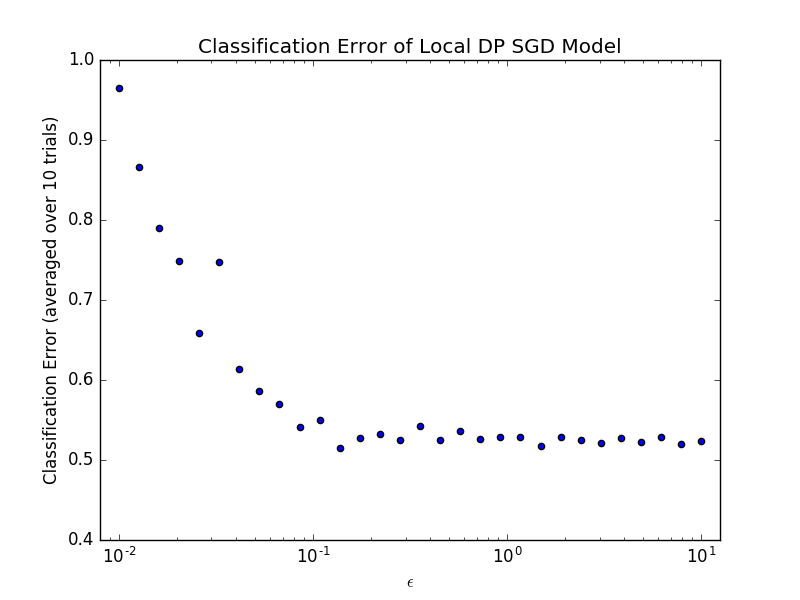
\includegraphics[scale=0.7]{classification_error.png}

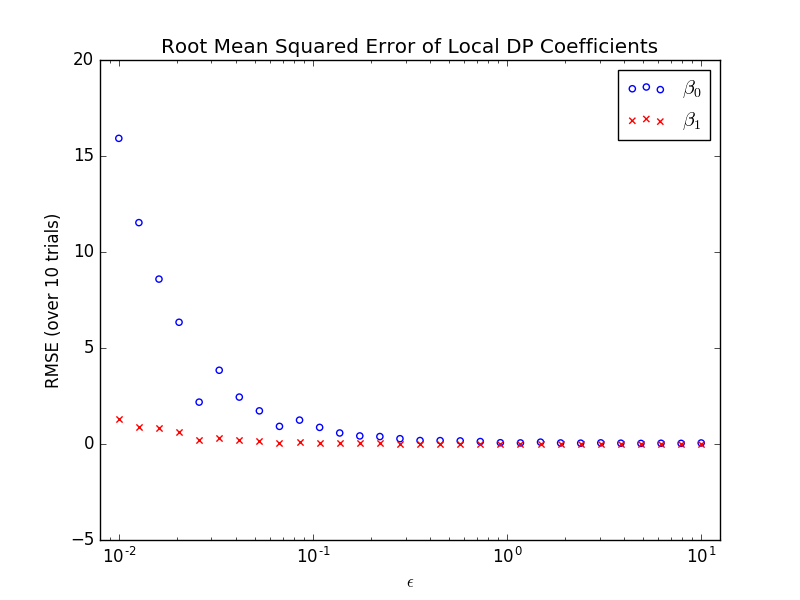
\includegraphics[scale=0.7]{rmse.png}

\subsection{Analysis}

\noindent

Looking at the results, we can see that the classification error predictably improves as $\epsilon$ increases, leveling off around $\epsilon = 0.1$. Interestingly, while the RMSE follows a similar trend, it takes longer to plateau, continuing to make small improvements as $\epsilon$ approaches $1$ and beyond. It makes sense that the classification error would plateau before the RMSE did, since the coefficients do not have to be exact for the classifier to work correctly. Also, since the classifier has fairly poor results (approximately 50/50 at predicting marriage based on education) even with non-private SGD, there is less to be gained by reducing the error since there is a lot of error intrinisic to the model.

\newpage

\begin{appendices}

\section{\cl{problem_2.py}}
\label{appendix:problem_2}

\begin{lstlisting}
import numpy as np
import csv
import matplotlib.pyplot as plt

# read in csv data
def read_data(file):
    with open(file, 'rb') as f:
        reader = csv.reader(f)
        next(f)
        X, Y = [], []
        for row in reader:
            try:
                X.append(int(row[4]))
                Y.append(int(row[9]))
            except:
                pass
        return np.array(X), np.array(Y)

# read in non-private coefficients
def read_non_private_coefs():
    with open('non_private_results.csv', 'rb') as f:
        reader = csv.reader(f)
        next(f)
        betas = []
        for row in reader:
            betas.append(float(row[1]))
        return np.array(betas)

# read in private coefficients
def read_private_coefs():
    with open('local_results.csv', 'rb') as f:
        reader = csv.reader(f)
        next(f)
        results = {}
        for row in reader:
            try:
                epsilon = float(row[1])
                results[epsilon] = np.vstack((results.get(epsilon, np.array([]).reshape(0, 2)), [float(row[2]), float(row[3])]))
            except:
                pass
        return results

# calculate classification error for given coefficient pair
def classification_error(X, Y, coef):
    num_correct = 0.
    for i in range(X.shape[0]):
        pred = coef[0] + coef[1] * X[i]
        num_correct += round(pred) == Y[i]
    return 1. - (num_correct / float(X.shape[0]))

# calculate average classification error for list of coefficient pairs
def calculate_avg_class_error(X, Y, coefs):
    avg_errors = {}
    for epsilon in sorted(coefs.keys()):
        errors = np.array([])
        for coef in coefs[epsilon]:
            errors = np.concatenate((errors, [classification_error(X, Y, coef)]))
        avg_errors[epsilon] = np.mean(errors, axis=0)
    return avg_errors

# plot the average classification error
def plot_avg_class_error(errors):
    X, Y = [], []
    for epsilon, error in errors.iteritems():
        X.append(epsilon)
        Y.append(error)

    plt.xscale('log')
    plt.scatter(X, Y)
    plt.xlabel(r'$\epsilon$')
    plt.ylabel('Classification Error (averaged over 10 trials)')
    plt.title('Classification Error of Local DP SGD Model')
    plt.xlim(min(X)/1.25, max(X)*1.25)
    plt.savefig('classification_error.png')
    plt.clf()

# calculate the rmse for two pairs of coefficients
def calculate_rmse(non_private_coef, private_coefs):
    avg_errors = {}
    for epsilon in sorted(private_coefs.keys()):
        errors = np.array([]).reshape(0, 2)
        for private_coef in private_coefs[epsilon]:
            errors = np.vstack((errors, [np.square(private_coef[0] - non_private_coef[0]), np.square(private_coef[1] - non_private_coef[1])]))
        avg_errors[epsilon] = np.sqrt(np.mean(errors, axis=0))
    return avg_errors

# plot the rmse
def plot_rmse(errors):
    X, Y_0, Y_1 = [], [], []
    for epsilon, error in errors.iteritems():
        X.append(epsilon)
        Y_0.append(error[0])
        Y_1.append(error[1])

    plt.xscale('log')
    plt.scatter(X, Y_0, label=r'$\beta_0$', edgecolors='blue', facecolors='none', marker='o')
    plt.scatter(X, Y_1, label=r'$\beta_1$', facecolors='red', marker='x')
    plt.xlabel(r'$\epsilon$')
    plt.ylabel('RMSE (over 10 trials)')
    plt.title('Root Mean Squared Error of Local DP Coefficients')
    plt.xlim(min(X)/1.25, max(X)*1.25)
    plt.legend(loc='upper right')
    plt.savefig('rmse.png')
    plt.clf()

def main():
    X, Y = read_data('MaPUMS5full.csv')

    non_private_coef = read_non_private_coefs()
    private_coefs = read_private_coefs()

    error = calculate_avg_class_error(X, Y, private_coefs)
    plot_avg_class_error(error)

    rmse = calculate_rmse(non_private_coef, private_coefs)
    plot_rmse(rmse)

if __name__ == "__main__":
    main()
\end{lstlisting}

\end{appendices}

\end{document}